\documentclass[aspectratio=169,10pt]{beamer}
\usepackage[english]{babel}\usepackage[utf8]{inputenc}\usepackage[T1]{fontenc}\usepackage{lmodern,booktabs,tabularx,tikz}\usetikzlibrary{arrows.meta,positioning}\usetheme{Madrid}
\definecolor{Ink}{HTML}{243748}\definecolor{Muted}{HTML}{667B8B}\definecolor{Accent}{HTML}{347E74}\definecolor{AccentBlue}{HTML}{507DAD}\definecolor{SoftMint}{HTML}{E6F4EE}\definecolor{SoftLilac}{HTML}{F1EEF8}\definecolor{Paper}{HTML}{FBFCFE}\setbeamercolor{background canvas}{bg=Paper}\setbeamercolor{normal text}{fg=Ink}\setbeamercolor{structure}{fg=Accent}\setbeamercolor{frametitle}{fg=Ink,bg=Paper}\setbeamercolor{footline}{fg=Muted,bg=Paper}\setbeamercolor{mintbox}{fg=Ink,bg=SoftMint}\setbeamercolor{lilacbox}{fg=Ink,bg=SoftLilac}\setbeamerfont{frametitle}{size=\large,series=\bfseries}\setbeamertemplate{headline}{}\setbeamertemplate{navigation symbols}{}\setbeamersize{text margin left=.48cm,text margin right=.48cm}
\setbeamertemplate{frametitle}{\nointerlineskip\begin{beamercolorbox}[wd=\paperwidth,ht=.74cm,dp=.14cm,leftskip=.55cm]{frametitle}\usebeamerfont{frametitle}\insertframetitle\end{beamercolorbox}}\setbeamertemplate{footline}{\begin{beamercolorbox}[wd=\paperwidth,ht=.30cm,dp=.16cm,rightskip=.48cm]{footline}\hspace{.48cm}\scriptsize Research Discussion\hfill\insertframenumber\,/\,\inserttotalframenumber\end{beamercolorbox}}
\newcommand{\card}[3]{\begin{beamercolorbox}[wd=\linewidth,rounded=true,sep=.11cm]{#1}{\small\bfseries\color{Accent}#2}\par\vspace{.04cm}{\footnotesize\raggedright #3\par}\end{beamercolorbox}}\newcommand{\lead}[1]{{\small\bfseries\color{Accent}#1\par\vspace{.04cm}}}\newcommand{\tagline}[1]{\vspace{.06cm}{\scriptsize\bfseries\color{AccentBlue}#1\par}}
\setlength{\emergencystretch}{1em}
\begin{document}
\begin{frame}[t]{Revised Research Scope}
{\small\color{Muted}Power- and Carbon-Aware LLM Serving in Heterogeneous GPU Racks\quad|\quad Research scope and candidate plan\par}\vspace{.10cm}\lead{Focus on single-server and single-rack serving before larger deployments.}
\begin{columns}[T,onlytextwidth]\begin{column}{.44\textwidth}\card{lilacbox}{Earlier scope}{Cross-data-center routing; WAN; HBM/HBF architecture exploration.}\end{column}\begin{column}{.53\textwidth}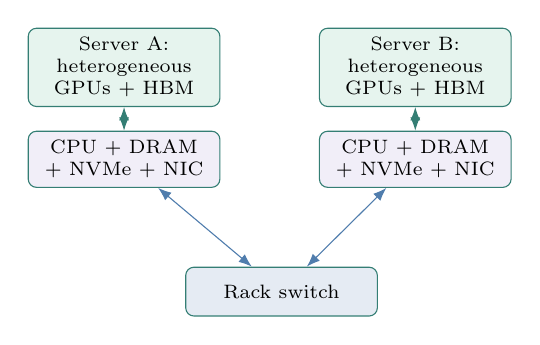
\begin{tikzpicture}[>=Latex,node distance=.3cm,box/.style={draw=Accent,fill=SoftMint,rounded corners=3pt,text width=2.2cm,minimum height=.62cm,align=center,font=\scriptsize}]\node[box](a){Server A: heterogeneous GPUs + HBM};\node[box,right=1.25cm of a](b){Server B: heterogeneous GPUs + HBM};\node[box,below=of a,fill=SoftLilac](c){CPU + DRAM + NVMe + NIC};\node[box,below=of b,fill=SoftLilac](d){CPU + DRAM + NVMe + NIC};\node[box,below=1cm of c,xshift=2cm,fill=AccentBlue!15](sw){Rack switch};\draw[<->,Accent](a)--(c);\draw[<->,Accent](b)--(d);\draw[<->,AccentBlue](c)--(sw);\draw[<->,AccentBlue](d)--(sw);\end{tikzpicture}\end{column}\end{columns}\vspace{.12cm}\card{mintbox}{Revised scope}{Multi-GPU server and multi-server rack; heterogeneous compute/HBM/bandwidth/power; HBM--DRAM--SSD hierarchy; chat, RAG, long-context, agentic workloads.}\vspace{.06cm}{\scriptsize Intra-server PCIe/NVLink where supported; rack Ethernet/InfiniBand/RDMA where deployed. WAN out of scope. NIC = network interface card; RDMA = remote direct memory access.\par}\tagline{Model placement and scheduling methods follow gap validation.}\end{frame}
\begin{frame}[t]{Power, Energy, and Carbon Metrics}
\lead{Optimize system energy under SLOs; retain full power and carbon accounting.}\begin{columns}[T,onlytextwidth]\begin{column}{.31\textwidth}\card{mintbox}{Power (W)}{Idle / baseline; dynamic / active; average; peak. Static power is not automatically measured idle power.}\end{column}\begin{column}{.32\textwidth}\card{lilacbox}{Energy (J, kWh)}{$E_{IT}=\int P_{IT}(t)dt$\par\vspace{.04cm}Operational energy; J/request; J/output token; J/completed task.}\end{column}\begin{column}{.33\textwidth}\card{mintbox}{Carbon}{Operational: $\sum_t E_{IT}(t)\,PUE(t)\,CI(t)$.\par\vspace{.04cm}Embodied carbon tracked separately over lifecycle. CI in gCO$_2$e/kWh when energy is kWh.}\end{column}\end{columns}\vspace{.10cm}\card{lilacbox}{Performance and power constraints}{TTFT, TPOT, SLO attainment, goodput, rack power budget.}\vspace{.10cm}\begin{beamercolorbox}[wd=\linewidth,sep=.09cm,rounded=true]{mintbox}\footnotesize At fixed CI and PUE, operational-carbon and energy rankings are identical. Embodied carbon is a lifecycle assessment, not runtime energy.\end{beamercolorbox}\end{frame}
\begin{frame}[t]{Previous Work and Candidate Research Gaps}
\lead{Prior studies provide complementary foundations; open questions need direct tests.}\small\renewcommand{\arraystretch}{1.25}\begin{tabularx}{\textwidth}{@{}>{\raggedright\arraybackslash}p{2.6cm}>{\raggedright\arraybackslash}X>{\raggedright\arraybackslash}X@{}}\toprule\textbf{Work}&\textbf{Established contribution}&\textbf{Question to validate}\\\midrule
GreenCache&Carbon-aware SSD KV sizing/replacement; DRAM/SSD power assumptions&Can activity-aware storage energy change decisions?\\
Carbon--SLO&Calibrated phase/batch energy and latency under SLOs&How does shared batch energy interact with tiered KV?\\
Kareto&Throughput/latency/cost-aware tier configuration&Are performance/cost optima also energy optima?\\
EcoServe&System-level operational/embodied accounting and design&How do serving activities affect energy and lifecycle accounting?\\\bottomrule\end{tabularx}\end{frame}
\begin{frame}[t]{Topic A: Workload-Aware Energy Optimization of Multi-Tier KV Cache}
{\small\color{Muted}Rank 1 | Primary candidate\par}\vspace{.05cm}\lead{Question: Can energy-aware cache choices reduce energy under latency SLOs?}\centering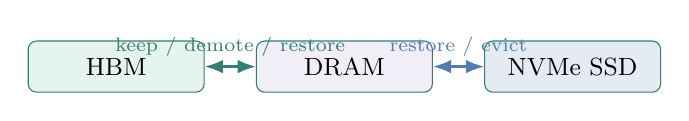
\begin{tikzpicture}[>=Latex,node distance=.65cm,box/.style={draw=Accent,fill=SoftMint,rounded corners=3pt,text width=2cm,minimum height=.65cm,align=center,font=\small}]\node[box](h){HBM};\node[box,right=of h,fill=SoftLilac](d){DRAM};\node[box,right=of d,fill=AccentBlue!15](s){NVMe SSD};\draw[<->,thick,Accent](h)--node[above,font=\scriptsize]{keep / demote / restore}(d);\draw[<->,thick,AccentBlue](d)--node[above,font=\scriptsize]{restore / evict}(s);\end{tikzpicture}\par\vspace{.08cm}\begin{columns}[T,onlytextwidth]\begin{column}{.49\textwidth}\card{mintbox}{Variables}{Capacity; prefix length; reuse probability/distance; request density; storage I/O; shared batch energy.}\end{column}\begin{column}{.49\textwidth}\card{lilacbox}{Research tests}{Does detailed energy change rankings? When is restore cheaper than recompute? Can policy save energy within SLO?}\end{column}\end{columns}\vspace{.08cm}\card{mintbox}{Feasibility}{Start single server. Verify SSD timing and profile needs first; expand to shared rack KV only if needed. SSD is not assumed to serve each active decode access.}\tagline{Potential contributions: calibrated model, break-even characterization, SLO-constrained policy (all to validate).}\end{frame}
\begin{frame}[t]{Topic B: Energy-Efficient Workload Scheduling on Heterogeneous GPU Racks}
{\small\color{Muted}Rank 2 | Alternative candidate\par}\vspace{.05cm}\lead{Question: Does KV locality and marginal batch energy improve GPU choice under SLOs?}\centering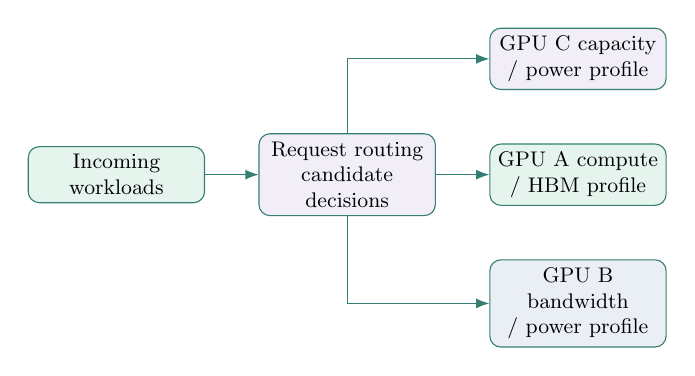
\begin{tikzpicture}[scale=.85,transform shape,>=Latex,node distance=.8cm,box/.style={draw=Accent,fill=SoftMint,rounded corners=4pt,text width=2.4cm,minimum height=.75cm,align=center,font=\small}]\node[box](w){Incoming workloads};\node[box,right=of w,fill=SoftLilac](r){Request routing candidate decisions};\node[box,right=of r](a){GPU A compute / HBM profile};\node[box,below=of a,fill=AccentBlue!12](b){GPU B bandwidth / power profile};\node[box,above=of a,fill=SoftLilac](c){GPU C capacity / power profile};\draw[->,Accent](w)--(r);\draw[->,Accent](r)--(a);\draw[->,Accent](r)|-(b);\draw[->,Accent](r)|-(c);\end{tikzpicture}\par\vspace{.10cm}\begin{columns}[T,onlytextwidth]\begin{column}{.49\textwidth}\card{mintbox}{Validate prior work}{DynamoLLM and FREESH already study energy-aware scheduling. Check their KV locality, shared-batch, host/storage, and communication models.}\end{column}\begin{column}{.49\textwidth}\card{lilacbox}{Initial boundary}{Start with fixed model/precision, existing replicas, and request routing. Defer heterogeneous TP/PP, layer placement, and phase disaggregation.}\end{column}\end{columns}\end{frame}
\begin{frame}[t]{Topic C: Energy-Aware KV Cache Management for Agentic LLM Serving}
{\small\color{Muted}Rank 3 | Workload-specific candidate\par}\vspace{.08cm}\lead{Question: Retain, move, or discard inactive session KV for later reuse?}\centering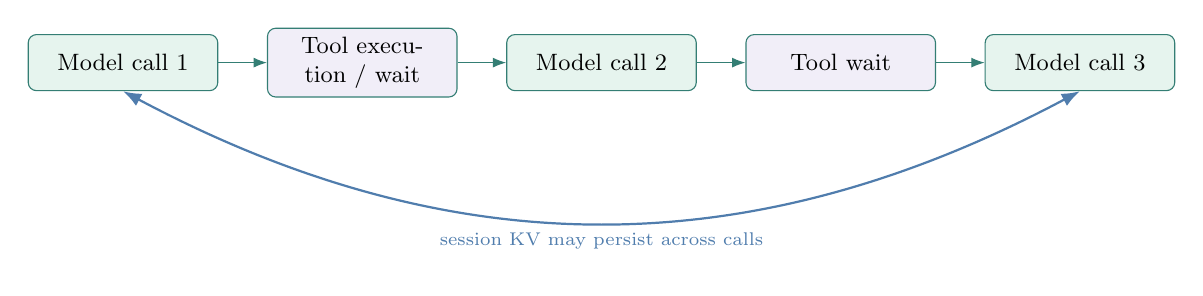
\begin{tikzpicture}[scale=.95,transform shape,>=Latex,node distance=.65cm,box/.style={draw=Accent,fill=SoftMint,rounded corners=3pt,text width=2.3cm,minimum height=.75cm,align=center,font=\small}]\node[box](m1){Model call 1};\node[box,right=of m1,fill=SoftLilac](t1){Tool execution / wait};\node[box,right=of t1](m2){Model call 2};\node[box,right=of m2,fill=SoftLilac](t2){Tool wait};\node[box,right=of t2](m3){Model call 3};\draw[->,Accent](m1)--(t1);\draw[->,Accent](t1)--(m2);\draw[->,Accent](m2)--(t2);\draw[->,Accent](t2)--(m3);\draw[<->,thick,AccentBlue](m1.south) to[bend right=28] node[below,font=\scriptsize]{session KV may persist across calls}(m3.south);\end{tikzpicture}\par\vspace{.08cm}\begin{columns}[T,onlytextwidth]\begin{column}{.49\textwidth}\card{mintbox}{Motivation}{Multi-turn calls, growing context, long residency, tool waits, session reuse.}\end{column}\begin{column}{.49\textwidth}\card{lilacbox}{Potential evidence}{Session energy; retention/offload behavior; energy per completed task. Verify public traces and tool timing. Separate inference energy from whole-agent energy and assess task quality.}\end{column}\end{columns}\tagline{Session-aware retention is not new. Topic C may be a workload within Topic A.}\end{frame}
\begin{frame}[t]{Research Gap Validation Plan}
\lead{Measure energy-related gaps before designing a new scheduling method.}\begin{columns}[T,onlytextwidth]\begin{column}{.32\textwidth}\card{mintbox}{1. Workload characterization}{Chat / RAG / agentic; input/output lengths; KV reuse; working set; session life and idle intervals.}\end{column}\begin{column}{.32\textwidth}\card{lilacbox}{2. Model fidelity}{Compare LLMServingSim power estimates and calibrated batch/storage/communication extensions against hardware measurements.}\end{column}\begin{column}{.32\textwidth}\card{mintbox}{3. Ranking comparison}{HBM only; HBM+DRAM; HBM+DRAM+SSD; recompute vs restore; performance-, cost-, and energy-oriented choices.}\end{column}\end{columns}\vspace{.12cm}\begin{beamercolorbox}[wd=\linewidth,sep=.12cm,rounded=true]{lilacbox}\small\bfseries\color{Accent}Core test\quad Does a more accurate system energy model change the ranking of feasible configurations or policies?\end{beamercolorbox}\vspace{.10cm}{\footnotesize Hold workload, hardware, policy, completed volume/observation horizon, and SLO constraints constant; vary the energy model. Any ranking reversal shown later must be labeled hypothetical. No outcomes are assumed.\par}\end{frame}
\begin{frame}[t]{Why LLMServingSim 2.0?}
\lead{A comprehensive, extensible foundation for heterogeneous serving research.}\begin{columns}[T,onlytextwidth]\begin{column}{.54\textwidth}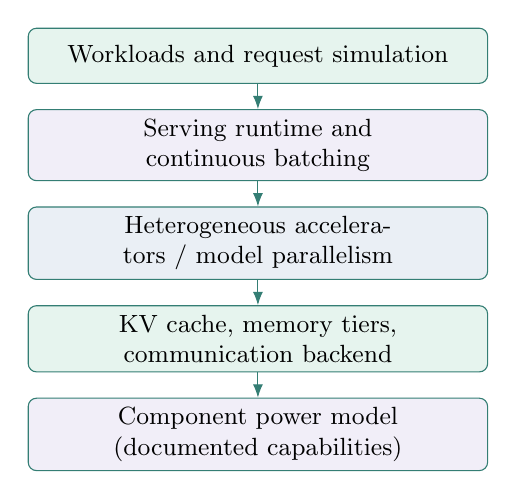
\begin{tikzpicture}[>=Latex,node distance=.32cm,box/.style={draw=Accent,fill=SoftMint,rounded corners=3pt,text width=5.6cm,minimum height=.7cm,align=center,font=\small}]\node[box](a){Workloads and request simulation};\node[box,below=of a,fill=SoftLilac](b){Serving runtime and continuous batching};\node[box,below=of b,fill=AccentBlue!12](c){Heterogeneous accelerators / model parallelism};\node[box,below=of c](d){KV cache, memory tiers, communication backend};\node[box,below=of d,fill=SoftLilac](e){Component power model (documented capabilities)};\draw[->,Accent](a)--(b);\draw[->,Accent](b)--(c);\draw[->,Accent](c)--(d);\draw[->,Accent](d)--(e);\end{tikzpicture}\end{column}\begin{column}{.42\textwidth}\card{mintbox}{Verified foundation}{Heterogeneous profiles; serving and network simulation; KV/memory features; documented node-level power fields.}\vspace{.10cm}\card{lilacbox}{Check version specifics}{Public docs and repo evolve. Audit pinned source, model coverage, component calibration, and feature flags before experiment design.}\vspace{.10cm}\card{mintbox}{Still to verify}{Storage idle-power field does not prove SSD cache timing, migration, or I/O contention.}\end{column}\end{columns}\vspace{.06cm}{\scriptsize Conceptual abstraction of framework; features vary by version. Paper: arXiv:2602.23036.\par}\end{frame}
\begin{frame}[t]{Proposed Power and Carbon Extensions}
\lead{Integrate calibrated component models into the existing simulation loop.}\centering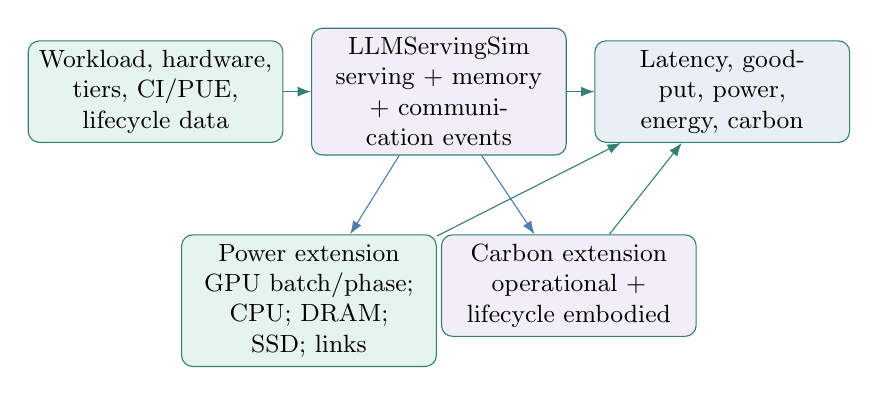
\begin{tikzpicture}[>=Latex,node distance=.35cm,box/.style={draw=Accent,fill=SoftMint,rounded corners=4pt,text width=3.0cm,minimum height=.8cm,align=center,font=\small}]\node[box](i){Workload, hardware, tiers, CI/PUE, lifecycle data};\node[box,right=of i,fill=SoftLilac](s){LLMServingSim serving + memory + communication events};\node[box,right=of s,fill=AccentBlue!12](o){Latency, goodput, power, energy, carbon};\node[box,below=1cm of s,xshift=-1.65cm](p){Power extension GPU batch/phase; CPU; DRAM; SSD; links};\node[box,below=1cm of s,xshift=1.65cm,fill=SoftLilac](c){Carbon extension operational + lifecycle embodied};\draw[->,Accent](i)--(s);\draw[->,Accent](s)--(o);\draw[->,AccentBlue](s)--(p);\draw[->,AccentBlue](s)--(c);\draw[->,Accent](p)--(o);\draw[->,Accent](c)--(o);\end{tikzpicture}\par\vspace{.07cm}\begin{columns}[T,onlytextwidth]\begin{column}{.49\textwidth}\card{mintbox}{Reuse model sources}{Carbon--SLO batch energy; DRAMPower / storage literature; GreenCache, EcoServe, ACT carbon methods; Kareto tier behavior.}\end{column}\begin{column}{.49\textwidth}\card{lilacbox}{Accounting safeguards}{Avoid adding request energy to shared batch energy; do not double-count GPU/HBM/base; apply PUE once; treat embodied carbon as lifecycle allocation, not runtime-avoided emissions.}\end{column}\end{columns}\vspace{.02cm}{\scriptsize Region-specific CI is a scenario input, not cross-data-center routing. Calibrate every refined model.\par}\end{frame}
\begin{frame}[t]{Proposed Next Steps}
\lead{Establish the evaluation framework before choosing an optimization method.}\begin{columns}[T,onlytextwidth]\begin{column}{.48\textwidth}\card{mintbox}{Phase 1 -- Survey}{Review power/carbon models; identify code, data, profiling sets; audit LLMServingSim 2.0.}\vspace{.08cm}\card{lilacbox}{Phase 2 -- Extend}{Reproduce baseline; extend energy accounting; add operational and embodied carbon; implement storage behavior only if audit finds gaps.}\end{column}\begin{column}{.48\textwidth}\card{mintbox}{Phase 3 -- Calibrate}{Validate against available measurements; characterize workloads and GPU/storage settings; compare energy and performance choices.}\vspace{.08cm}\card{lilacbox}{Phase 4 -- Select topic}{Validate gaps; choose a feasible research question; then design the necessary method.}\end{column}\end{columns}\vspace{.10cm}\begin{beamercolorbox}[wd=\linewidth,sep=.10cm,rounded=true]{mintbox}\small\bfseries\color{Accent}Discussion\quad Is Topic A the right starting point? Single server or multi-server first? Which traces and hardware are available? Which model extensions are essential?\end{beamercolorbox}\end{frame}
\end{document}
